\lecture{Risolvere il Problema della Cinematica Inversa}{10~-~06~-~2026}
%

%
\section{L'Asimmetria Fondamentale della Cinematica e gli Ostacoli Matematici}
\emph{Questa sezione introduce la profonda differenza tra i due problemi della cinematica e i vincoli analitici della cinematica inversa (IK)}.
\begin{description}
    \item [Cinematica Diretta (Forward Kinematics)] Riceve come input gli angoli dei giunti ($q$) e calcola in modo lineare la posa cartesiana dell'end-effector ($x, y, z$). Si tratta di una mappatura diretta che restituisce sempre un'unica soluzione univoca (problema considerato intuitivo e ``facile'').
    \item [Cinematica Inversa (Inverse Kinematics)] Riceve come input la posa cartesiana desiderata dell'end-effector e deve ricavare gli angoli dei giunti richiesti per raggiungerla. Rappresenta una complessa ricerca di configurazioni valide all'interno di uno spazio multidimensionale (problema considerato ``difficile'').
\end{description}
%
\subsection{I tre Ostacoli Matematici della Cinematica Inversa}
Troviamo tre problemi fondamentali riguardo la cinematica inversa:
\begin{enumerate}
    \item \textbf{Non-linearità}: Le equazioni di posa sono governate da funzioni trascendenti accoppiate (seni e coseni nelle matrici di rotazione), impedendo una semplice inversione algebrica lineare.
    \item \textbf{Molteplicità}: Una singola posizione cartesiana dell'end-effector può essere raggiunta attraverso configurazioni geometriche multiple del braccio robotico (fino a 8 combinazioni distinte per un robot a 6 assi).
    \item \textbf{Singolarità}: Configurazioni geometriche critiche in cui il determinante della matrice Jacobiana si annulla ($\det(J)=0$), provocando la perdita istantanea di uno o più gradi di libertà.
\end{enumerate}
Vedi figura \ref{fig:ikhurd}\ref{sub@fig:ik1},\ref{sub@fig:ik2},\ref{sub@fig:ik3}.
\begin{figure}
    \centering
    \begin{subfigure}{0.45\linewidth}
        \centering
        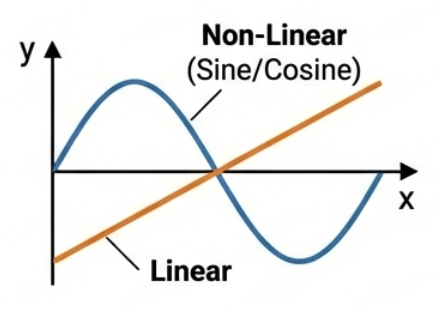
\includegraphics[width=\linewidth]{assets/ik1.png}
        \caption{Non-Linearity}\label{fig:ik1}
    \end{subfigure}
    \begin{subfigure}{0.45\linewidth}
        \centering
        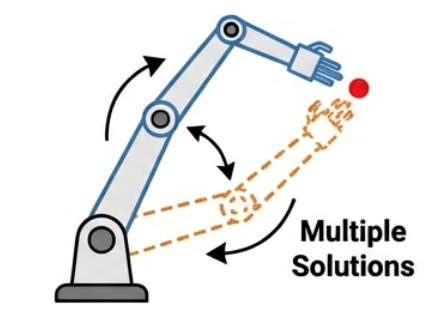
\includegraphics[width=\linewidth]{assets/ik2.png}
        \caption{Multiplicy}\label{fig:ik2}
    \end{subfigure}
    \begin{subfigure}{0.45\linewidth}
        \centering
        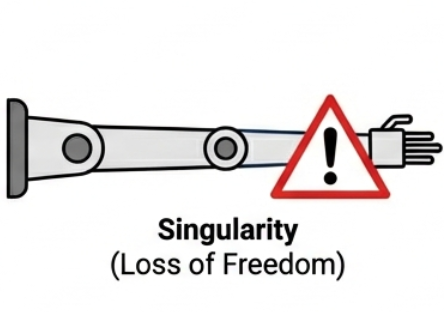
\includegraphics[width=\linewidth]{assets/ik3.png}
        \caption{Singularity}\label{fig:ik3}
    \end{subfigure}
    \caption{The 3 Mathematical Hurdles of Inverse Kinematics}\label{fig:ikhurd}
\end{figure}

%
\section{Risoluzione dei problemi: Metodi Analitici e Numerici}
L'inversione matematica della catena cinematica può essere affrontata seguendo due filosofie opposte.
%
\subsection{Metodi Analitici (Closed-Form)}
Sviluppano una derivazione geometrica o algebrica esatta del sistema di equazioni.
\begin{description}
    \item [Vantaggi] Sono computazionalmente rapidissimi in tempo reale e hanno la capacità intrinseca di calcolare contemporaneamente tutte le soluzioni ammissibili.
    \item [Svantaggi] Sono strettamente specifici per l'architettura di un determinato robot e risultano difficili o impossibili da ricavare per geometrie irregolari o complesse.
    \item [Approcci] Si suddividono in approccio geometrico (basato sull'intuizione spaziale e su teoremi trigonometrici come il Teorema del Coseno) e approccio algebrico (basato sulla manipolazione diretta e l'isolamento delle variabili nelle matrici di trasformazione).
\end{description}

%
\subsection{Metodi Numerici (Iterativi)}
Utilizzano algoritmi di approssimazione matematica ad appuntamenti successivi, come l'algoritmo di Newton-Raphson.
\begin{description}
    \item [Vantaggi] Hanno una validità generale (lo stesso algoritmo si applica a qualsiasi struttura di robot) e riescono a gestire agevolmente i robot cinematicamente ridondanti.
    \item [Svantaggi] Sono computazionalmente più lenti, calcolano una sola soluzione per volta e soffrono del rischio di convergere in minimi locali errati.
    \item [Principio] Calcolano lo scostamento (errore $dx$) nello spazio cartesiano e utilizzano la matrice Jacobiana inversa ($J^{-1}$) per aggiornare progressivamente la velocità e la posizione dei giunti fino a quando l'errore non si azzera ($\dot{q}=J^{-1}\dot{x}$).
\end{description}

%
\section{Il Caso di Studio UR3 e il Disaccoppiamento Cinematico}
\begin{description}
    \item [Caratteristiche Meccaniche] Si tratta di un cobot a 6 gradi di libertà (6-DOF) composto da una catena seriale di bracci rigidi collegati da giunti rotoidi.
    \item [Geometria del Polso Disassato] L'UR3 presenta una configurazione sfalsata del polso (Offset Wrist) che definisce accuratamente la sua tabella dei parametri DH (Denavit-Hartenberg).
    \item [Il Disaccoppiamento Cinematico] Questa specifica conformazione permette di semplificare il problema matematico a 6 variabili, separandolo in due sottoproblemi più piccoli e indipendenti:
          \begin{enumerate}
              \item Braccio di posizionamento (joints 1, 2, 3): Ha il compito esclusivo di muovere la struttura per determinare la coordinata spaziale tridimensionale del centro del polso (Wrist Center Location);
              \item Polso di orientamento (joints 4, 5, 6): Riceve la posizione fissa del centro del polso e si occupa unicamente di calcolare la rotazione angolare finale dell'end-effector.
          \end{enumerate}
          \begin{figure}
              \centering
              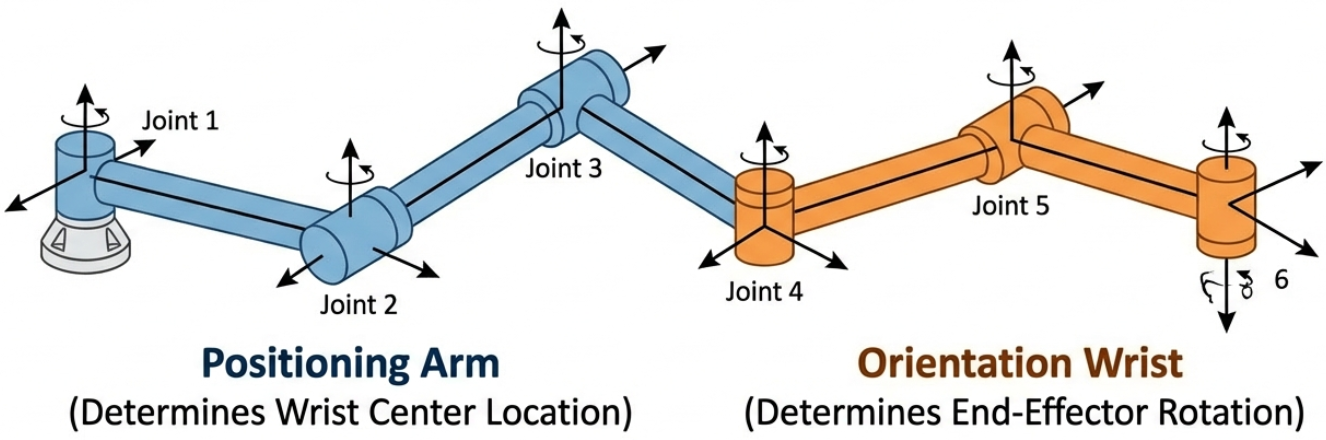
\includegraphics[width=\linewidth]{assets/ik4.png}
              \caption{Kinematic Decoupling}\label{fig:kindec}
          \end{figure}
          Vedi figura \ref{fig:kindec}.
\end{description}

%
\subsection{Algoritmo di Risoluzine Analitica}
Questa sezione descrive la pipeline matematica utilizzata dal controller per calcolare analiticamente gli angoli di giunto.
\begin{description}
    \item [Step 1: Risoluzione della Base (Giunto 1)] Si proietta la coordinata cartesiana del centro del polso ($P_x, P_y$) sul piano bidimensionale $ XY $ della base del robot. Questo passaggio svela geometricamente due soluzioni d'allineamento valide, note come configurazione a ``Spalla Sinistra'' (Left Shoulder) o ``Spalla Destra'' (Right Shoulder). La formula risolutiva è:
          \[
              \theta_1 = \text{atan2}(P_y, P_x) \pm \text{Correction}
          \]
    \item [Step 2: Risoluzione del Centro del Polso (Giunto 5)] Sfruttando la geometria costruttiva ad assi paralleli dell'UR3, il Giunto 5 definisce l'angolo di beccheggio (pitch) del polso rispetto al piano della base. L'equazione di riferimento è:
          \[
              P_x \sin(\theta_1) - P_y \cos(\theta_1) = d_4
          \]
          Risolvendo questa relazione si isolano due scenari di rotazione simmetrica (soluzione positiva o negativa):
          \[
              \theta_{5}=\tan^{-1}\frac{C_{234}(C_{1}a_{x}+S_{1}a_{y})+S_{234}a_{z}}{S_{1}a_{x}-C_{1}a_{y}}
          \]
    \item [Step 3: Risoluzione del Braccio Planare (Giunti 2, 3 e 4)] Avendo bloccato i valori della base e del polso, la porzione centrale del robot si riduce a un problema planare bidimensionale a 3 bracci (struttura a triangolo).

          Il controller applica il Teorema del Coseno per estrarre l'angolo del gomito $\theta_3$:
          \[
              \theta_{3}=\tan^{-1}\frac{S_{3}}{C_{3}}
          \]
          Successivamente determina l'angolo della spalla $\theta_2$ calcolandolo in base all'altezza e al raggio della terna cartesiana:
          \[
              \theta_2 = \tan^{-1}\frac{(C_3a_3+a_2)(P_z-S_{234}a_{4})-S_3a_3(P_xC_1+P_yS_1-C_{234}a_{4})}{(C_3a_3+a_2)(P_xC_1+P_y-C_{234}a_{4})+S_3a_3(P_z-S_{234}a_{4})}
          \]
\end{description}

%
\section{Criteri di Selezione delle Molteplicità e Implementazione Software}
\begin{description}
    \item [Le 8 Configurazioni Spaziali] A causa della presenza di formule quadratiche e di radici quadrate trigonometriche inversibili ($\pm$), una singola posa cartesiana obiettivo genera fino a 8 percorsi di movimento geometricamente corretti (es. combinazioni di Elbow Up, Elbow Down, Wrist Flipped e Wrist Unflipped).
    \item [Criterio di Minimo Spostamento ($\Delta q$)] Per impedire movimenti improvvisi, erratici o scatti pericolosi dei motori, il software di controllo seleziona tassativamente l'unica soluzione geometrica che minimizza la distanza angolare totale ($\Delta q$) rispetto alla posizione corrente in cui si trova il robot.
    \item [Implementazione Pratica] Nello sviluppo software moderno, librerie dedicate come Robotics Toolbox for Python automatizzano la modellizzazione DH e i calcoli cinematici inversi (utilizzando ad esempio funzioni numeriche come l'algoritmo di Levenberg-Marquardt \verb|ikine_LM|).
    \item [Ingegnerizzazione Industriale] Per i manipolatori industriali di precisione come l'UR3, le soluzioni analitiche in forma chiusa rimangono nettamente superiori rispetto alle varianti numeriche, in quanto garantiscono la massima velocità di calcolo deterministica e la certezza matematica di mappare tutti i set di soluzioni presenti.
\end{description}